\section{Biography Section}
\vspace{-8mm}

% \bf{If you include a photo:}
\begin{IEEEbiography}
[\vspace{-6mm}{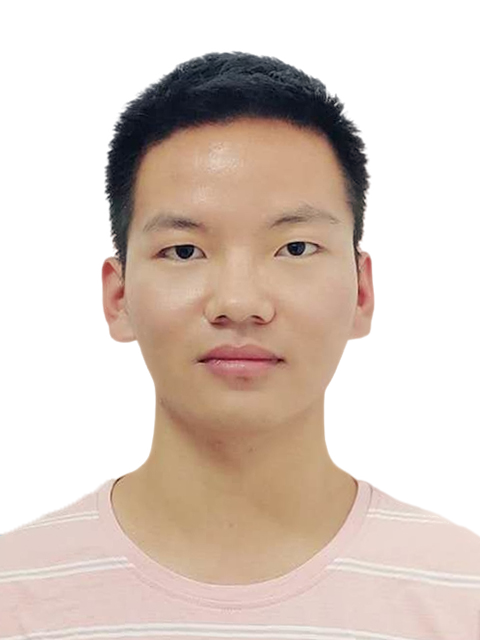
\includegraphics[width=1in,height=1.25in,clip,keepaspectratio]{images/biography_photo/chenglong_wang.png}}]{Chenglong Wang}
is currently working toward a Ph.D. degree in computer science at Northeastern University, Shenyang, China. His research interests include deep reinforcement learning and efficient alignment training for natural language generation. He is a Member of the Northeastern University Natural Language Processing Laboratory.
\end{IEEEbiography}
\vspace{-10mm}
\begin{IEEEbiography}
[\vspace{-6mm}{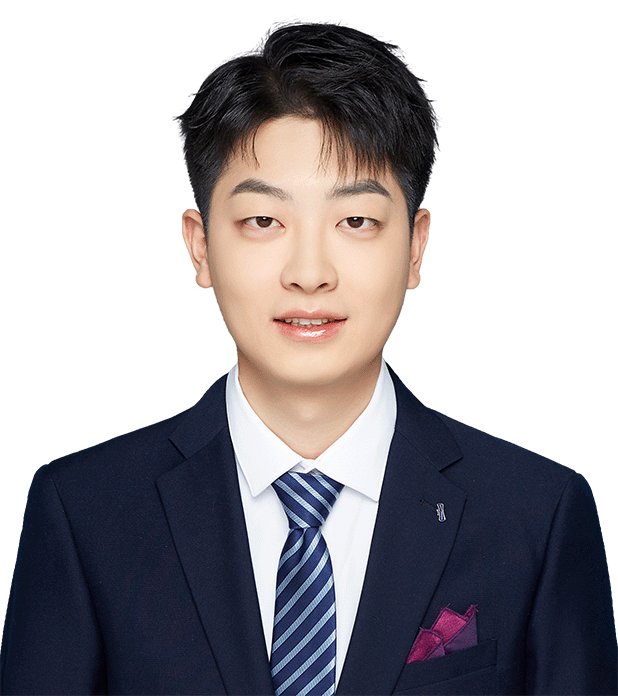
\includegraphics[width=1in,height=1.25in,clip,keepaspectratio]{images/biography_photo/hang_zhou.png}}]{Hang Zhou}
received a bachelor's degree in Computer Science and Technology from Northeastern University, Shenyang, China, where he is currently a member of the Natural Language Processing Laboratory, working towards a master’s degree in 2022. His research interests include deep reinforcement learning for natural language generation.
\end{IEEEbiography}
\vspace{-10mm}
\begin{IEEEbiography}
[\vspace{-7mm}{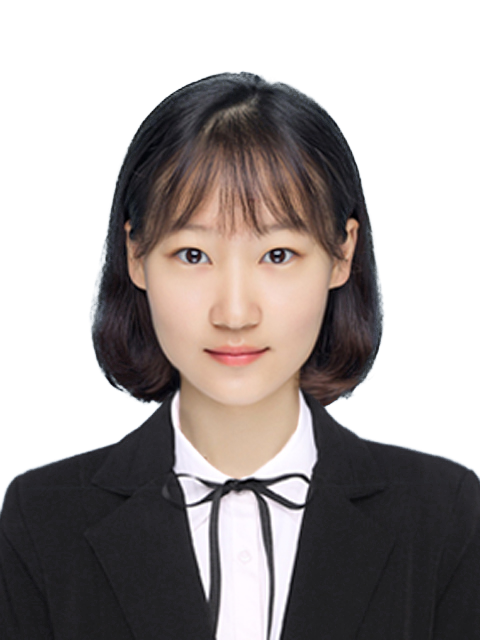
\includegraphics[width=1in,height=1.25in,clip,keepaspectratio]{images/biography_photo/kaiyan_chang.png}}]{Kaiyan Chang}
is currently working toward a master’s degree in computer science and technology from Northeastern University, Shenyang, China. Her research interests include efficient prompt methods and deep reinforcement learning for large language models. She is a Member of the Northeastern University Natural Language Processing Laboratory.
\end{IEEEbiography}
\vspace{-10mm}
\begin{IEEEbiography}
[\vspace{-1.5mm}{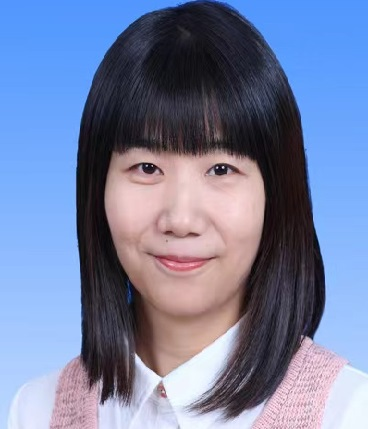
\includegraphics[width=1in,height=1.25in,clip,keepaspectratio]{images/biography_photo/tongran_liu.jpg}}]{Tongran Liu}
was born in 1982. She received the Ph.D. degree in Psychology from Chinese Academy of Sciences, Beijing, China, in 2009. She has been with Institute of Psychology, Chinese Academy of Sciences, since 2009. She is currently an associate professor with Institute of Psychology, Chinese Academy of Sciences. She has published more than 20 papers. Her current research interests include the neural mechanisms of human's cognitive control and reinforcement learning processes.
\end{IEEEbiography}
\vspace{-10mm}
\begin{IEEEbiography}
[\vspace{-6mm}{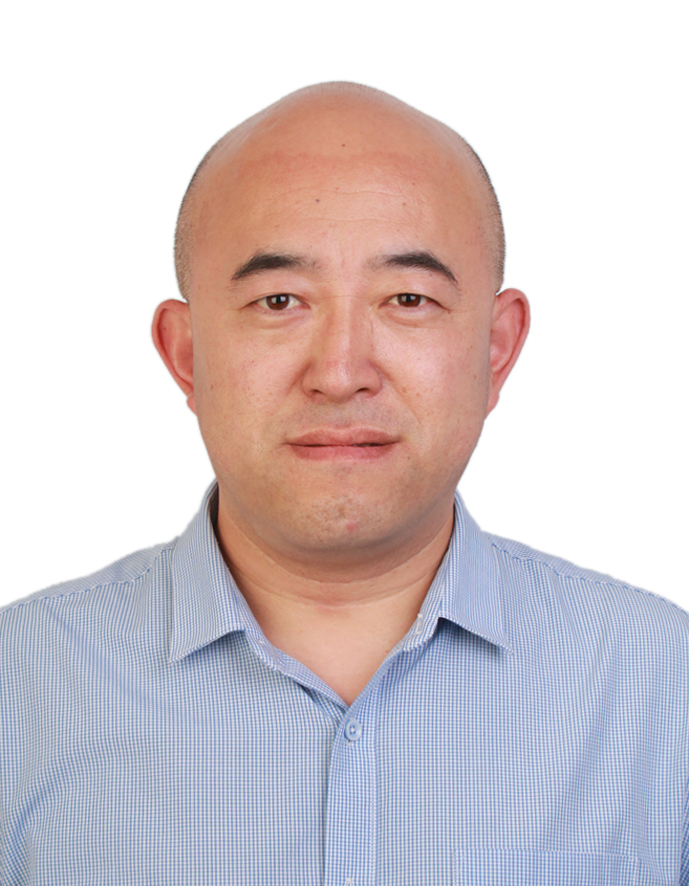
\includegraphics[width=1in,height=1.25in,clip,keepaspectratio]{images/biography_photo/chunliang_zhang.png}}]{Chunliang Zhang}
was born in 1973. He received his master’s degree in applied linguistics from Jilin University, Changchun, China in 2001. He is currently an asscoiate professor with Foreign Languages Studies, Northeastern University, and he has co-authored over 20 NLP-related papers during his 17 years’ collaboration with the Natural Language Processing Laboratory. His current interest is machine translation.
\end{IEEEbiography}
\vspace{-10mm}
\begin{IEEEbiography}
[\vspace{-5mm}{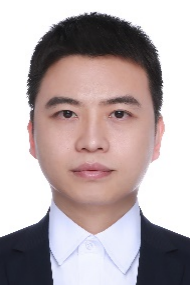
\includegraphics[width=1.4in,height=1.25in,clip,keepaspectratio]{images/biography_photo/murun_yang.png}}]{Murun Yang}
is currently working toward the Ph.D. degree in Computer Science and Technology with the Northeastern University, Shenyang, China. His research interests include text style transfer and machine translation. He is a member of the Northeastern University Natural Language Processing Laboratory.
\end{IEEEbiography}
\vspace{-10mm}
\begin{IEEEbiography}
[\vspace{-0mm}{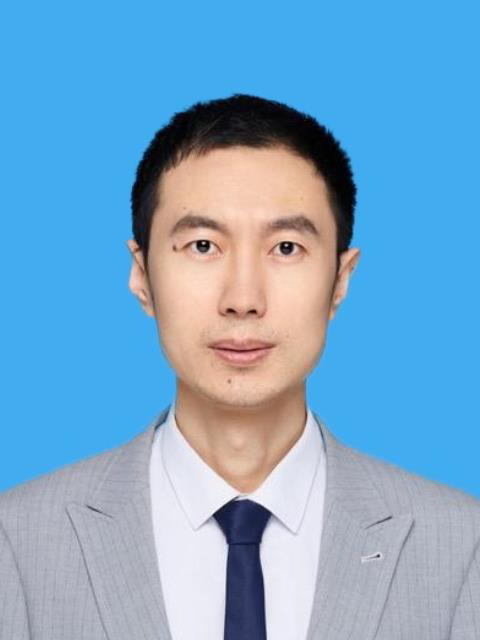
\includegraphics[width=1in,height=1.25in,clip,keepaspectratio]{images/biography_photo/quan_du.png}}]{Quan Du}
received the Bachelor's, Master's, and Ph.D. degrees in computer science all from Northeastern University, Shenyang, China, in 2012, 2014, and 2022, respectively. He is currently working in the NiuTrans team of Shenyang YaTrans Network Technology Co., Ltd. as the chief technology officer, in charge of the research and development of machine translation technology and products. His main research interests include machine translation, natural language processing and deep learning. 
\end{IEEEbiography}
\vspace{-10mm}
\begin{IEEEbiography}
[\vspace{-0mm}{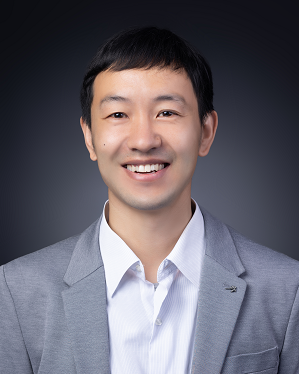
\includegraphics[width=1in,height=1.25in,clip,keepaspectratio]{images/biography_photo/tong_xiao.png}}]{Tong Xiao}
is a Professor in the College of Computer Science and Engineering at Northeastern University. His research interests include natural language processing and machine learning. He has contributed to several open-source NLP systems, such as the NiuTrans machine translation system. He led a team that has achieved top rankings several times in evaluations like WMT, NTCIR, and CCMT. He served as the PC chair for CCMT 2020 and as an area chair or senior area chair for several top-tier conferences, including ACL, EMNLP, and COLING. His work has been recognized with best paper awards and nominations at CCL 2018 and NLPCC 2024.
\end{IEEEbiography}
\vspace{-10mm}
\begin{IEEEbiography}
[\vspace{-0mm}{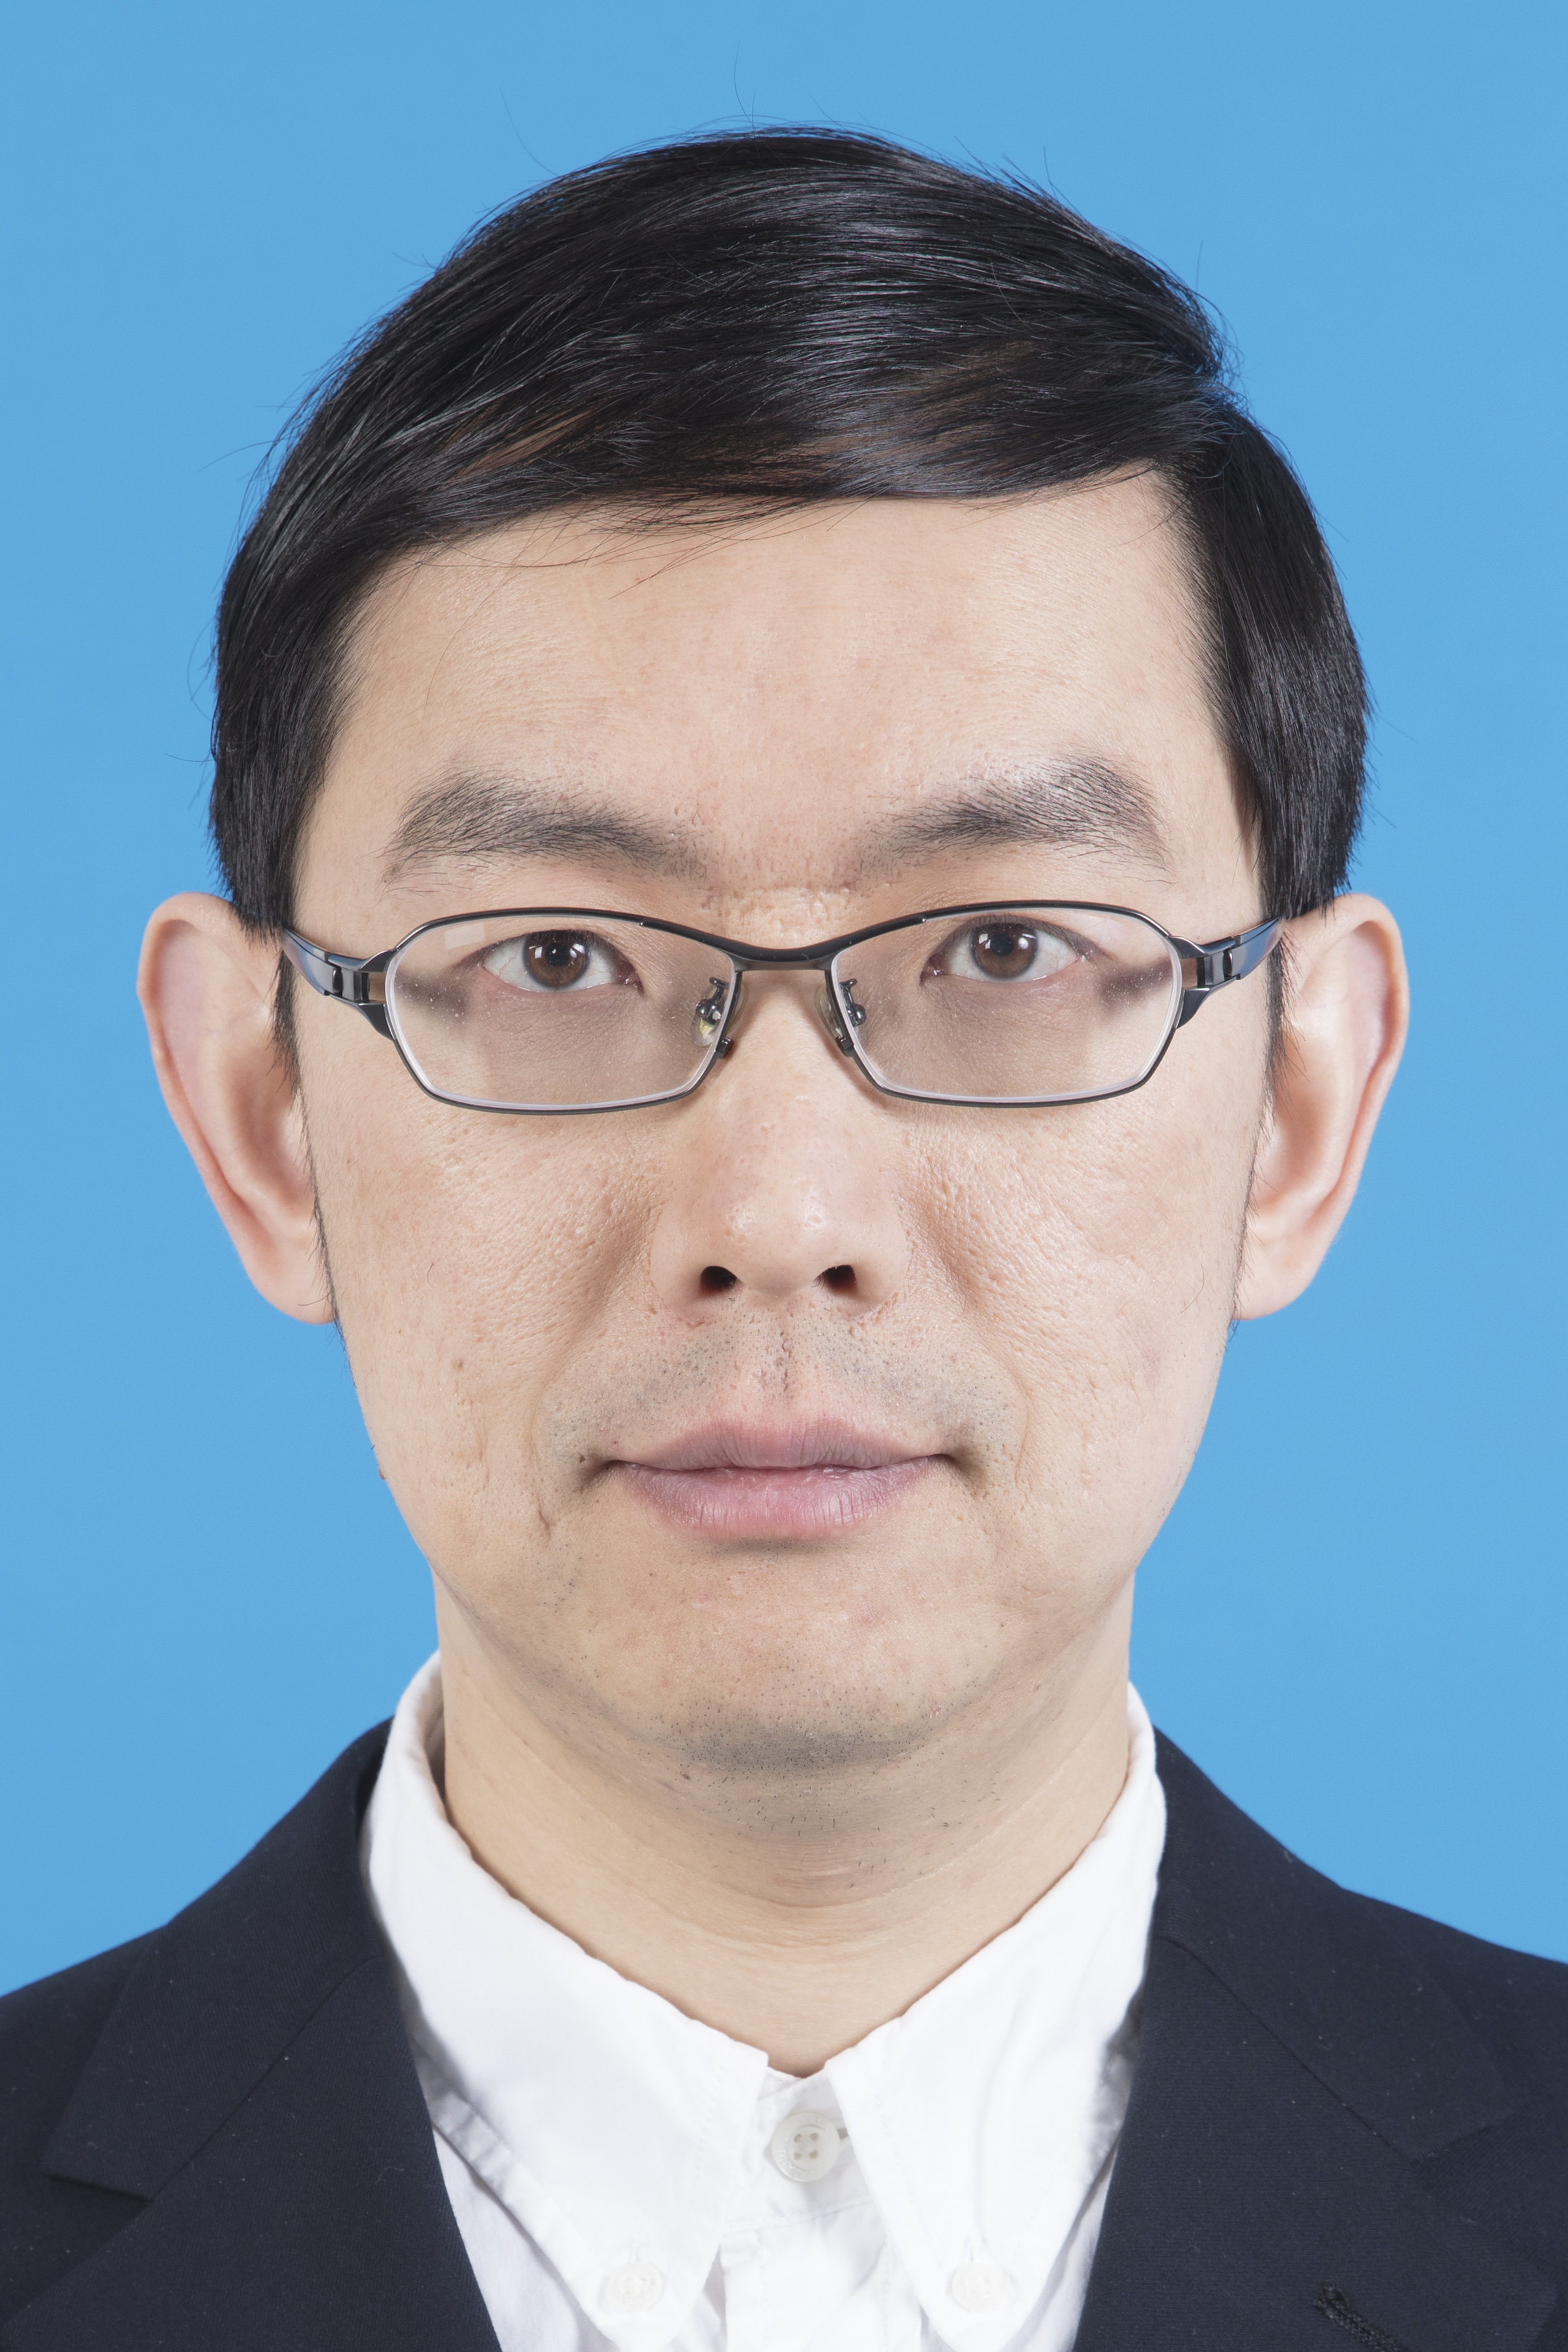
\includegraphics[width=1in,height=1.25in,clip,keepaspectratio]{images/biography_photo/yue_zhang.jpg}}]{Yue Zhang}
is a tenured Professor at Westlake University. His research interests include NLP and its underlying machine learning algorithms. His major contributions to the field include psycholinguistically motivated machine learning algorithm, learning-guided beam search for structured prediction, pioneering neural NLP models including graph LSTM, and OOD generalization for NLP. He authored the Cambridge University Press book ``Natural Language Processing -- a Machine Learning Perspective''. He is the PC co-chair for CCL 2020 and EMNLP 2022, and action editor for Transactios for ACL. He also served as associate editor for IEEE/ACM Transactions of Audio Speech and Language Processing (TASLP), ACM Transactions on Asian and Low-Resource Languages (TALLIP), IEEE Transactions on Big Data (TBD) and Computer, Speech and Language (CSL). He won the best paper awards of IALP 2017 and COLING 2018, best paper honorable mention of SemEval 2020, and best paper nomination for ACL 2018 and ACL 2023.
\end{IEEEbiography}
\vspace{-10mm}
\begin{IEEEbiography}
[\vspace{-0mm}{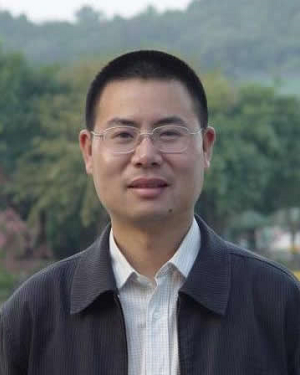
\includegraphics[width=1in,height=1.25in,clip,keepaspectratio]{images/biography_photo/jingbo_zhu.png}}]{Jingbo Zhu}
received the Ph.D. degree in computer science from Northeastern University, Shenyang, China, in 1999. He has been with Northeastern University, since 1999. He is currently a Full Professor with the College of Computer Science and Engineering and is in charge of research activities with the Natural Language Processing Laboratory. He has published more than 180 papers and holds four U.S. patents. His current research interests include syntactic parsing, machine translation, and machine learning for natural language processing.
\end{IEEEbiography}
